%%%%%%%%%% Aquí va el código.
\subsection*{Pregunta 2.} La siguiente tabla define los tokens para un lenguaje simple donde
$\Sigma = \{a, \dotsm, z, 0, \dotsm, 9, \oplus, (, )\}$
\begin{center}
  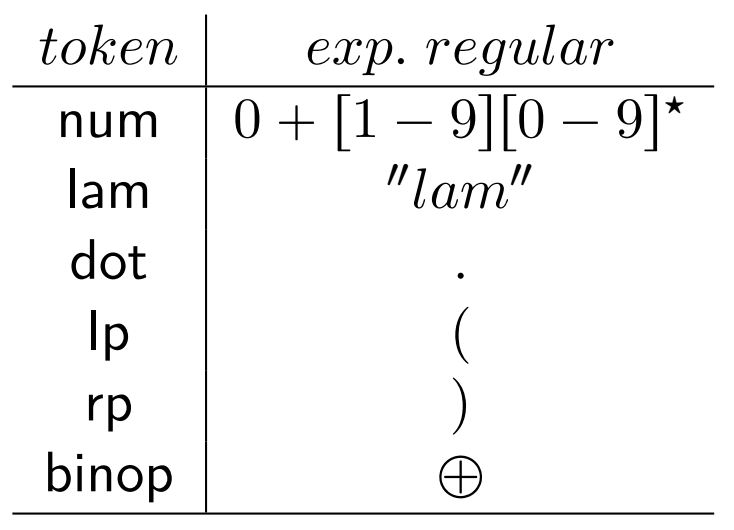
\includegraphics[scale=0.20]{./Tabla.png}
\end{center}
\begin{itemize}
\item[$a$)] Extiende la tabla anterior para agregar un token para identificadores donde la
  primera letra debe ser mayúscula seguida de cualquier secuencia de letras o números.
\item[$b$)] Construye un autómata finito determinista que acepte los tokens descritos en la tabla.
  Puedes usar algún método, eg. derivadas de expresiones regulares o construcción de un $AFN_{\epsilon}$ y
  transformaciones. Indica el método usado y muestra el proceso.
\end{itemize}
